\documentclass{standalone}
\usepackage{tikz}
\usetikzlibrary{matrix,arrows,decorations.pathmorphing,decorations.pathreplacing,calc,positioning}
\usepackage{xcolor}
% all other packages and stuff you need for the picture
\newcommand{\myunit}{0.65 cm}
\newcommand{\myraise}{3pt}
\tikzset{
    lpltsty/.style={decorate, decoration = {brace,mirror,raise=3pt,amplitude=5pt}},
    namesty/.style={pos=0.5,below=7pt},
    scalarsty/.style={draw,fill=white,rectangle,minimum size=\myunit,anchor=center},
    indexsty/.style={fill,fill=white,rectangle,minimum width=\myunit,anchor=center},
    touchsty/.style={fill,fill=red,rectangle,minimum size=\myunit},
    ycsty/.style={fill,fill=yellow,rectangle,minimum size=\myunit},
    brcsty/.style={fill,fill=brown,rectangle,minimum size=\myunit},
    blcsty/.style={fill,fill=cyan!20,rectangle,minimum size=\myunit},
    becsty/.style={fill,fill=beige,rectangle,minimum size=\myunit},
    ocsty/.style={fill,fill=orange,rectangle,minimum size=\myunit},
    whclsty/.style={fill,fill=white,rectangle,minimum size=\myunit},
    zcsty/.style={fill,fill=white,rectangle,minimum size=\myunit,text=zerogray},
    nzsty/.style={fill,fill=black,rectangle,minimum size=\myunit,text=white},
    rcsty/.style={fill,fill=purple,rectangle,minimum size=\myunit},
    pcsty/.style={fill,fill=pink,rectangle,minimum size=\myunit},
    lcsty/.style={fill,fill=blue,rectangle,minimum size=\myunit},
    bcsty/.style={fill,fill=black,rectangle,minimum size=\myunit, text=white},
    hlsty/.style={draw=red},
}


\colorlet{zerogray}{gray!25}
\colorlet{beige}{brown!70}

\newcommand{\ylcl}{|[ycsty]|1}
\newcommand{\recl}{|[rcsty]|2}
\newcommand{\picl}{|[pcsty]|3}
\newcommand{\blcl}{|[blcsty]|1}
\newcommand{\brcl}{|[brcsty]|2}
\newcommand{\becl}{|[becsty]|3}
\newcommand{\orcl}{|[ocsty]|4}
\newcommand{\bkcl}{|[bcsty]|5}
\newcommand{\whcl}{|[whclsty]|0}
\newcommand{\zecl}{|[zcsty]|0}

\newcommand{\formatscale}{0.5}
\newcommand{\matrixscale}{0.69}
\begin{document}

\resizebox{\linewidth}{!}{%
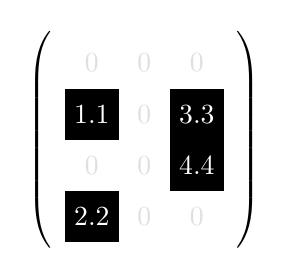
\begin{tikzpicture}[>=latex]
\matrix (A) [matrix of math nodes,
  nodes = {whclsty},
  left delimiter  = (,
  right delimiter = ),
  ampersand replacement=\&] at (0,0)
{
\zecl \& \zecl \& \zecl\\
|[nzsty]|1.1 \& \zecl \& |[nzsty]|3.3 \\
\zecl \& \zecl \& |[nzsty]|4.4\\
|[nzsty]|2.2 \& \zecl \& \zecl\\
};
\end{tikzpicture}%
}
\resizebox{2.0\linewidth}{!}{%
\begin{tikzpicture}[>=latex]

\node (Aif) at (0, 0) {SubFiber(... position=1)};

\matrix (A) [matrix of math nodes,
  nodes = {whclsty},
  left delimiter  = (,
  right delimiter = ),
  ampersand replacement=\&,
  anchor=north,
  below=\myraise of Aif]
{
|[fullsty]| \& |[fullsty]| \& |[fullsty]| \\
};

\node (Ai1f) [anchor=north, below left = 2*\myunit and 2*\myunit of A.south west] {SubFiber(=1)};
\draw (A-1-1.center) -- (Ai1f.north) node [midway, fill=white] {$i=1$};
\matrix (Ai1) [matrix of math nodes,
  nodes = {whclsty},
  left delimiter  = (,
  right delimiter = ),
  ampersand replacement=\&,
  anchor=north,
  below=\myraise of Ai1f.south]
{
\zecl \& |[fullsty]| \& \zecl \& |[fullsty]|\\
};

\node (Ai2f) [right = \myunit of Ai1f.east] {SubFiber(lvl2, pos=2)};
\draw (A-1-2.center) -- (Ai2f.north) node [midway, fill=white] {$i=2$};
\matrix (Ai2) [matrix of math nodes,
  nodes = {whclsty},
  left delimiter  = (,
  right delimiter = ),
  ampersand replacement=\&,
  anchor = north,
  below = \myraise of Ai2f.south]
{
\zecl \& \zecl \& \zecl \&  \zecl \\
};

\node (Ai3f) [right = \myunit of Ai2f.east] {SubFiber(lvl2, pos=3)};
\draw (A-1-3.center) -- (Ai3f.north) node [midway, fill=white] {$i=3$};
\matrix (Ai3) [matrix of math nodes,
  nodes = {whclsty},
  left delimiter  = (,
  right delimiter = ),
  ampersand replacement=\&,
  anchor = north,
  below = \myraise of Ai3f.south]
{
\zecl \& |[fullsty]| \& |[fullsty]| \&  \zecl \\
};

\node (A21f) [anchor=north, below = 2*\myunit of Ai1-1-2, nzsty] {1.1};
\draw (Ai1-1-2.center) -- (A21f.north) node [midway, fill=white] {$i =2$};
\node (A41f) [anchor=north, below = 2*\myunit of Ai1-1-4, nzsty] {2.2};
\draw (Ai1-1-4.center) -- (A41f.north) node [midway, fill=white] {$i=4$};

\node (A23f) [anchor=north, below = 2*\myunit of Ai3-1-2, nzsty] {3.3};
\draw (Ai3-1-2.center) -- (A23f.north) node [midway, fill=white] {$i=2$};
\node (A33f) [anchor=north, below = 2*\myunit of Ai3-1-3, nzsty] {4.4};
\draw (Ai3-1-3.center) -- (A33f.north) node [midway, fill=white] {$i=3$};

\end{tikzpicture}%
}

\end{document}